\documentclass{myhw}
\linespread{1.05}        % Palatino needs more leading (space between lines)
\usepackage{extarrows}
\usepackage{mathrsfs}
\usepackage{braket}
\titleformat{\section}[runin]{\sffamily\bfseries}{}{}{}[]
\titleformat{\subsection}[runin]{\sffamily\bfseries}{}{}{}[]
\renewcommand{\exname}{Question }
\renewcommand{\subexcounter}{(\alph{homeworkSectionCounter})}
\newcommand{\id}{\text{Id}}
\newcommand{\tr}{\text{Tr}}
\newcommand{\rib}{\text{Rib}}

\title{CSC 2515 Homework 3}
\begin{document}

%% Question 1
\begin{homeworkProblem}
\textbf{Multilayer Perceptron.} \\
\emph{Give the weights and biases of a multilayer perceptron which takes as input two scalar values $(x_1,x_2)$ and outputs the values in sorted order. The hidden units should all use the ReLU activation function, and the output units should be linear. You should explain why your solution works, but you don’t need to provide a formal proof.} \\
\\
The multilayer perceptron after removing the lines with a weight of 0 is shown in Figure \ref{fig:q1.1}. 
\begin{figure}[h]
  \centering
  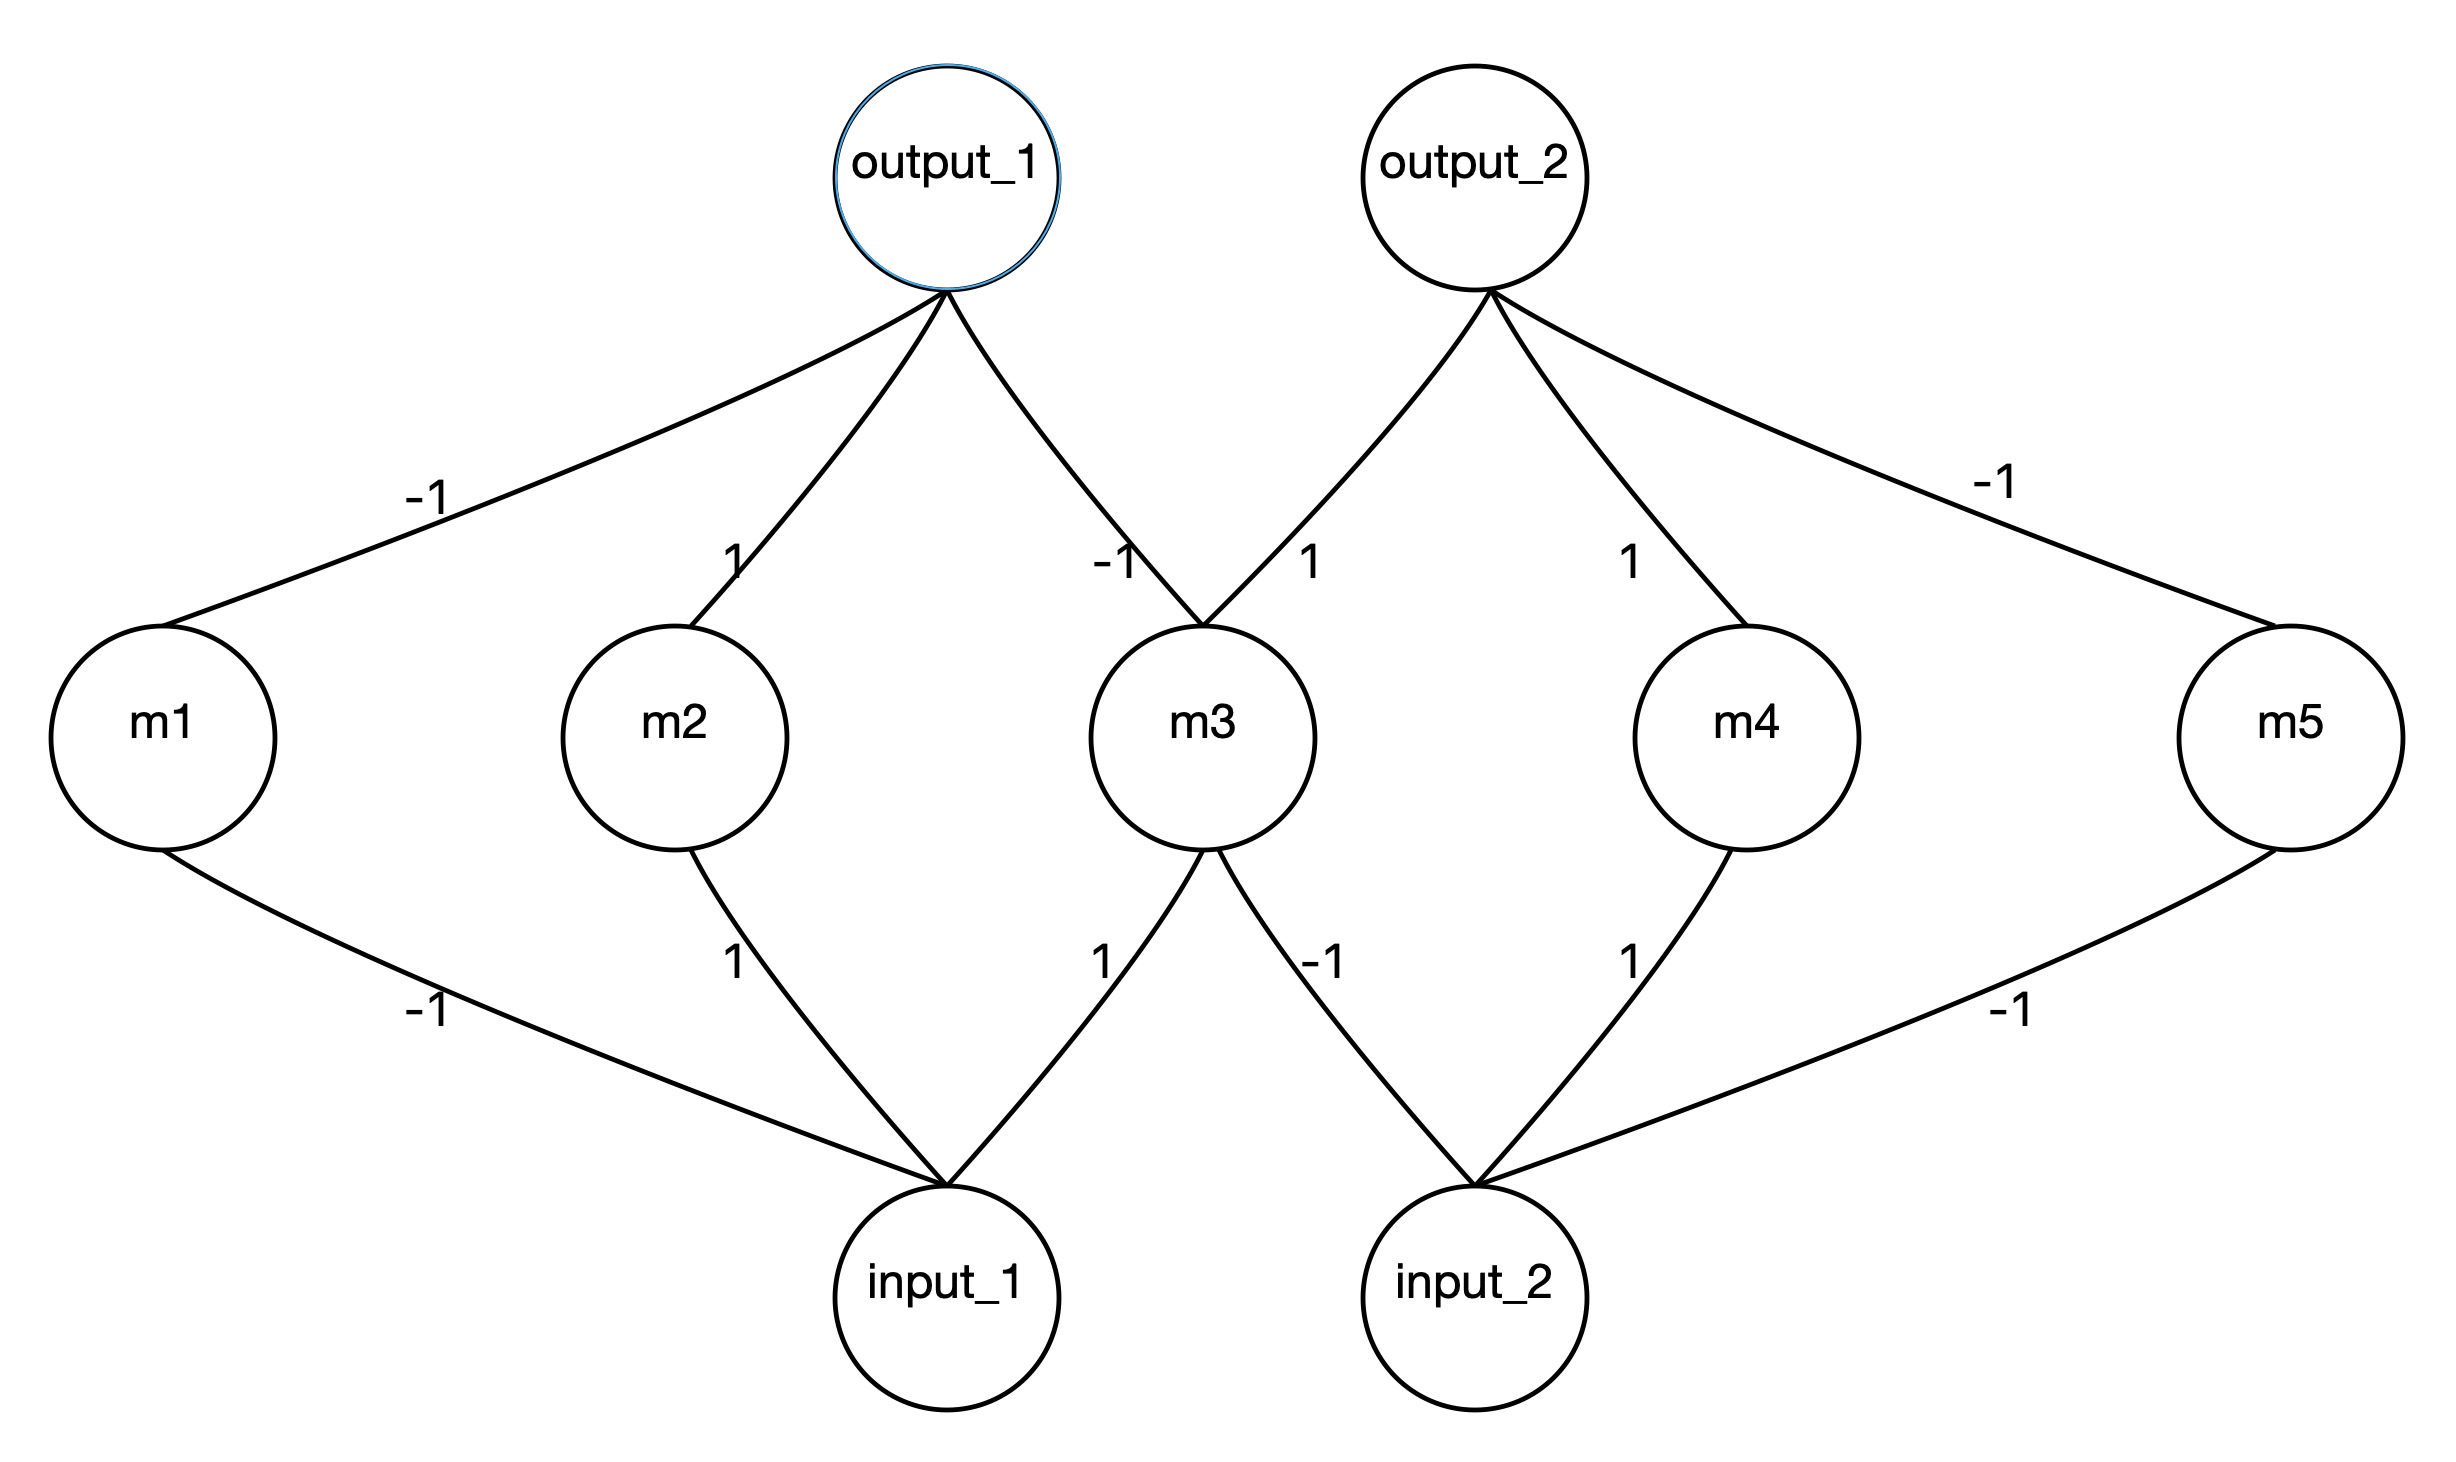
\includegraphics[width=.5\textwidth]{q1.2.png} 
  \caption{The multilayer perceptron without 0-weight lines. }
  \label{fig:q1.1}
\end{figure}
\\
$input_1$ and $input_2$ is the input of two values. $output_1$ is the less number of the input values and $output_2$ is the greater one.
$m_1$ to $m_5$ shows the hidden units with ReLU as their activation function. All biases are 0.
\\
\\
For simple cases, where $input_1$ and $input_2$ are both greater than or equal to 0, $m_1$ and $m_5$ will both be 0 and $m_2$ is a copy of $input_1$; similarly, $m_4$ is a copy of $input_2$. $m_3$ calculates $(input_1 - input_2)$. When $input_1 \ge input_2$, $m_3$ will be a positive number, $(input_1 - input_2)$. Then, $output_1$ will be $input_1 - (input_1 - input_2) = input_2$, which is the less number. $output_2$ will be $input_2 + (input_1 - input_2) = input_1$. When $input_1 < input_2$, $m_3$ will become 0. Then, $output_1$ will be $input_1$, which is the less number, and $output_2$ will be $input_2$.
\\
\\
For the cases where $input_1$ and $input_2$ can be negative numbers. The role of $m_1$ is to store the value of $input_1$ instead of $m_2$ when $input_1$ is less than 0, where $m_2$ will be 0 according to the ReLU activation function.
\\
\\
The complete multilayer perceptron is shown in Figure \ref{fig:q1.2}.
\begin{figure}[h]
  \centering
  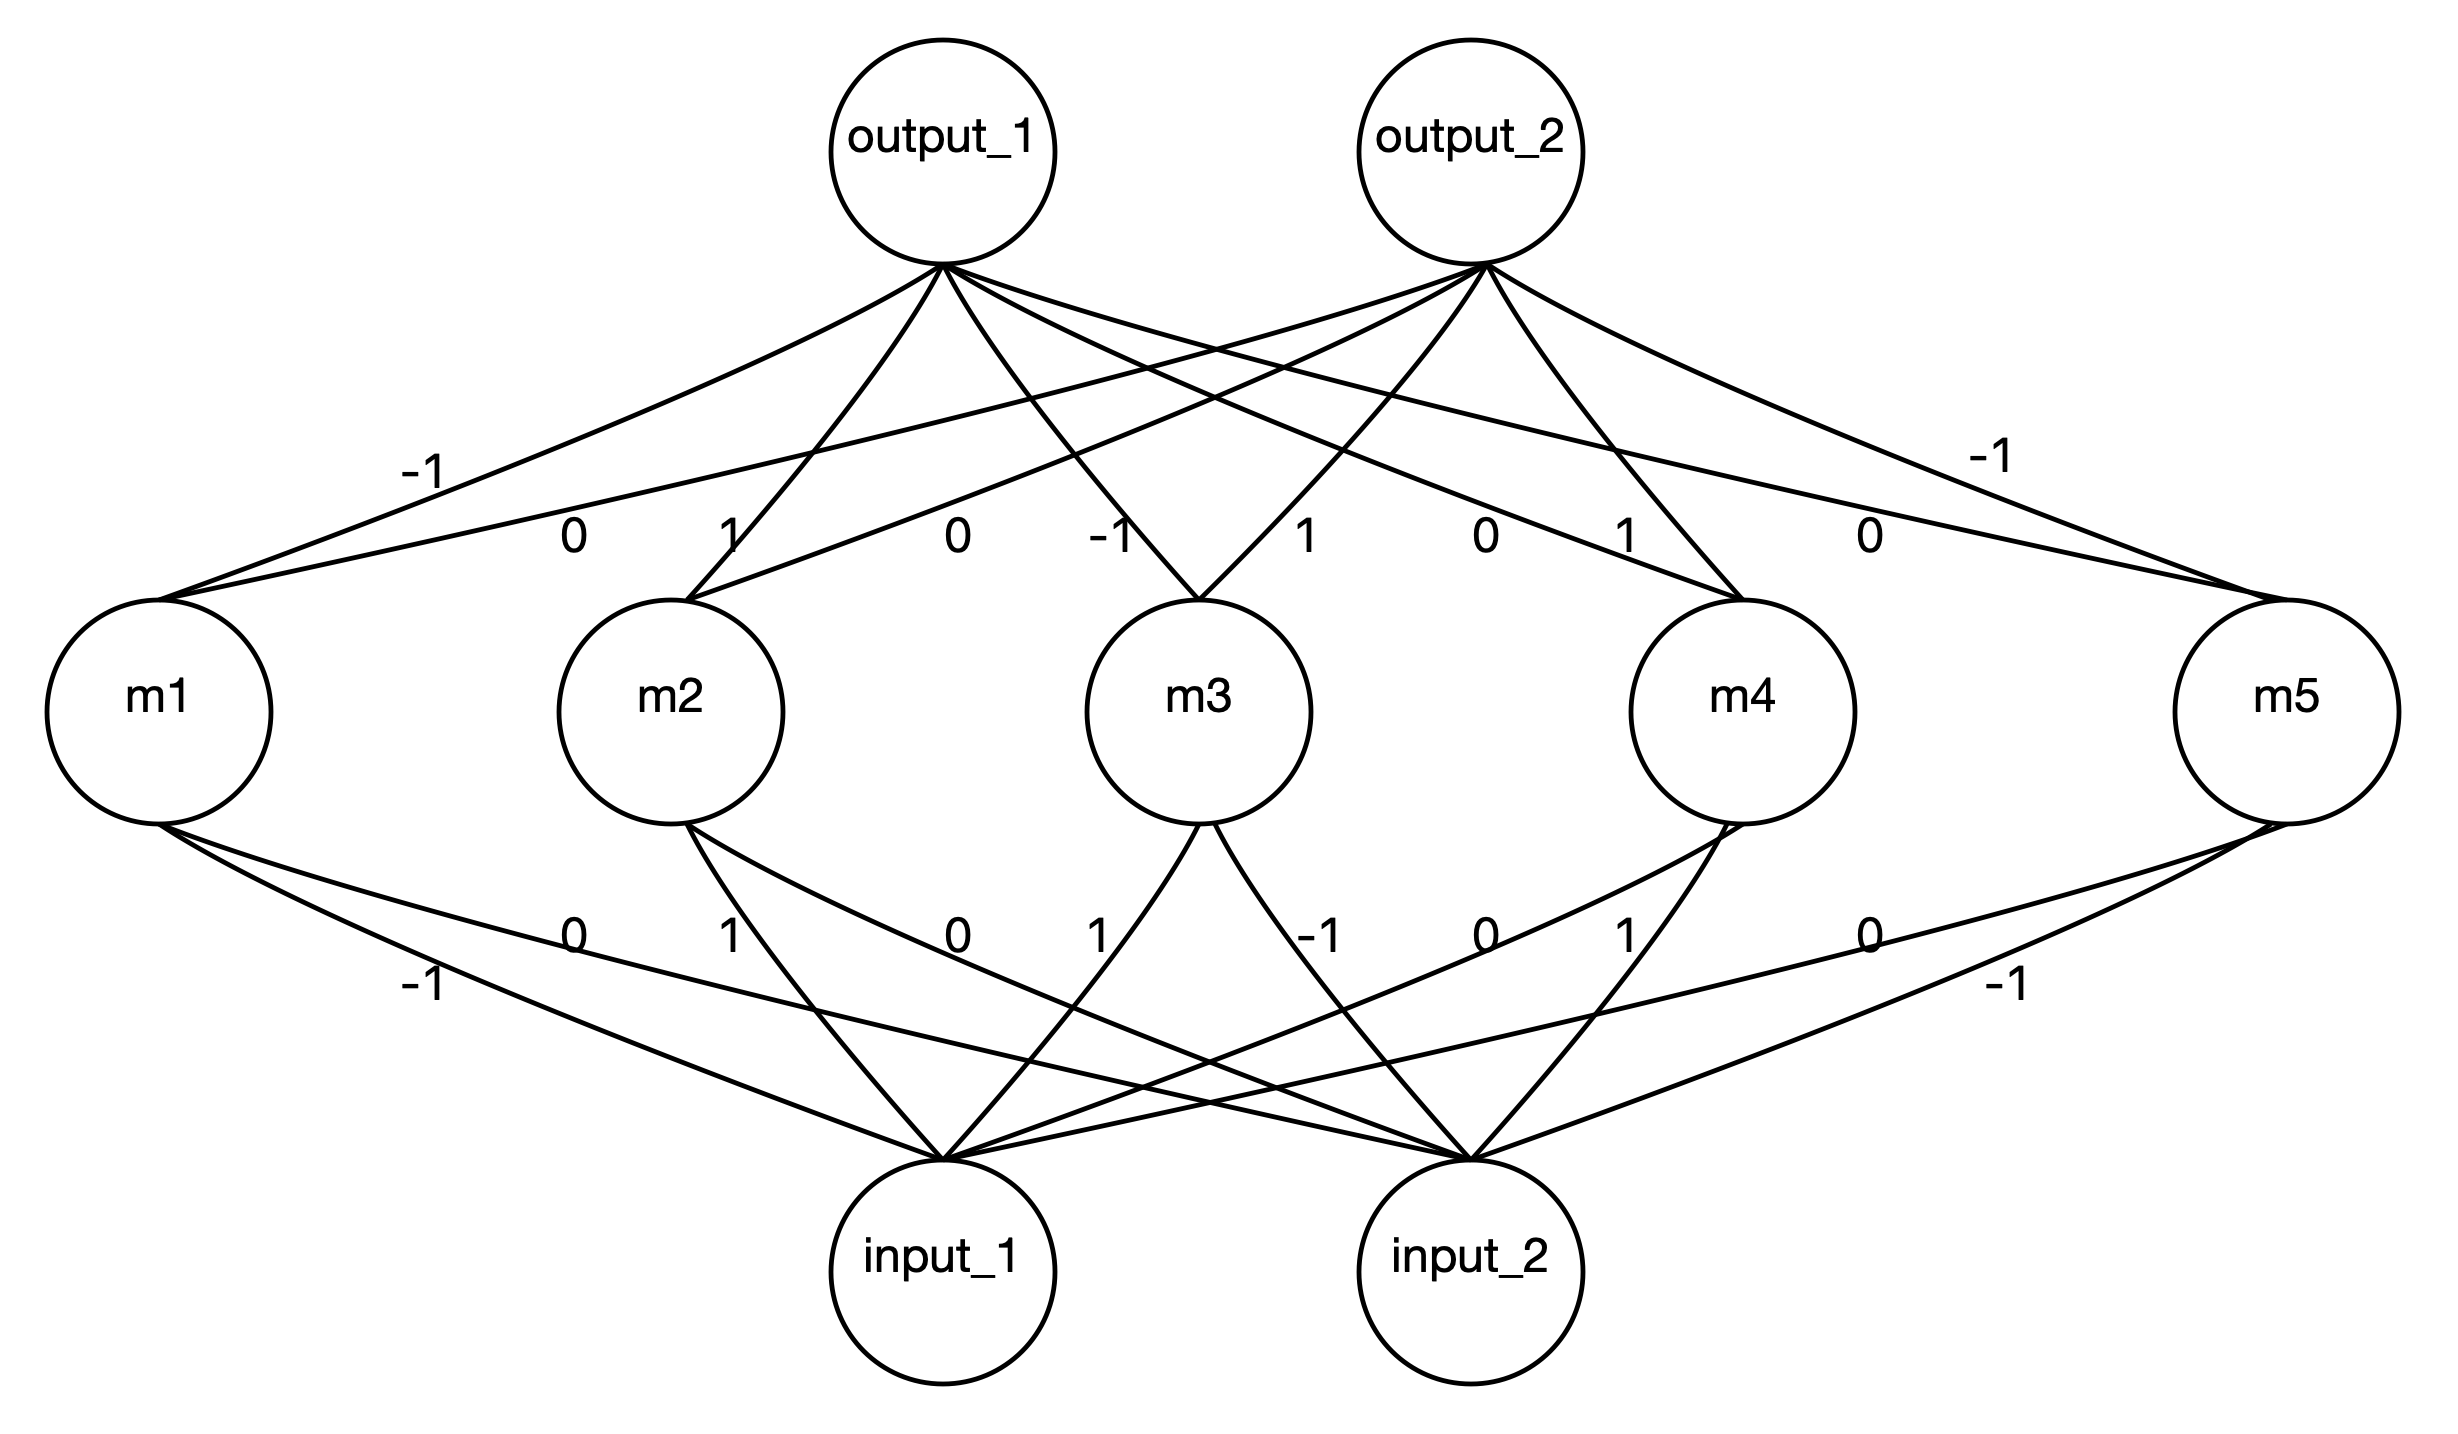
\includegraphics[width=.5\textwidth]{q1.3.png} 
  \caption{The multilayer perceptron for sorting input values. The hidden units use the ReLU activation function, and the output units are linear. }
  \label{fig:q1.2}
\end{figure}
\end{homeworkProblem}


%% Question 2
\begin{homeworkProblem}
\textbf{Backprop.}
%%% Subquestion 1
\begin{homeworkSection}
\emph{Draw the computation graph for all the variables.} \\
\\
The computation graph is shown in Figure \ref{fig:q2.1}.
\begin{figure}[h]
  \centering
  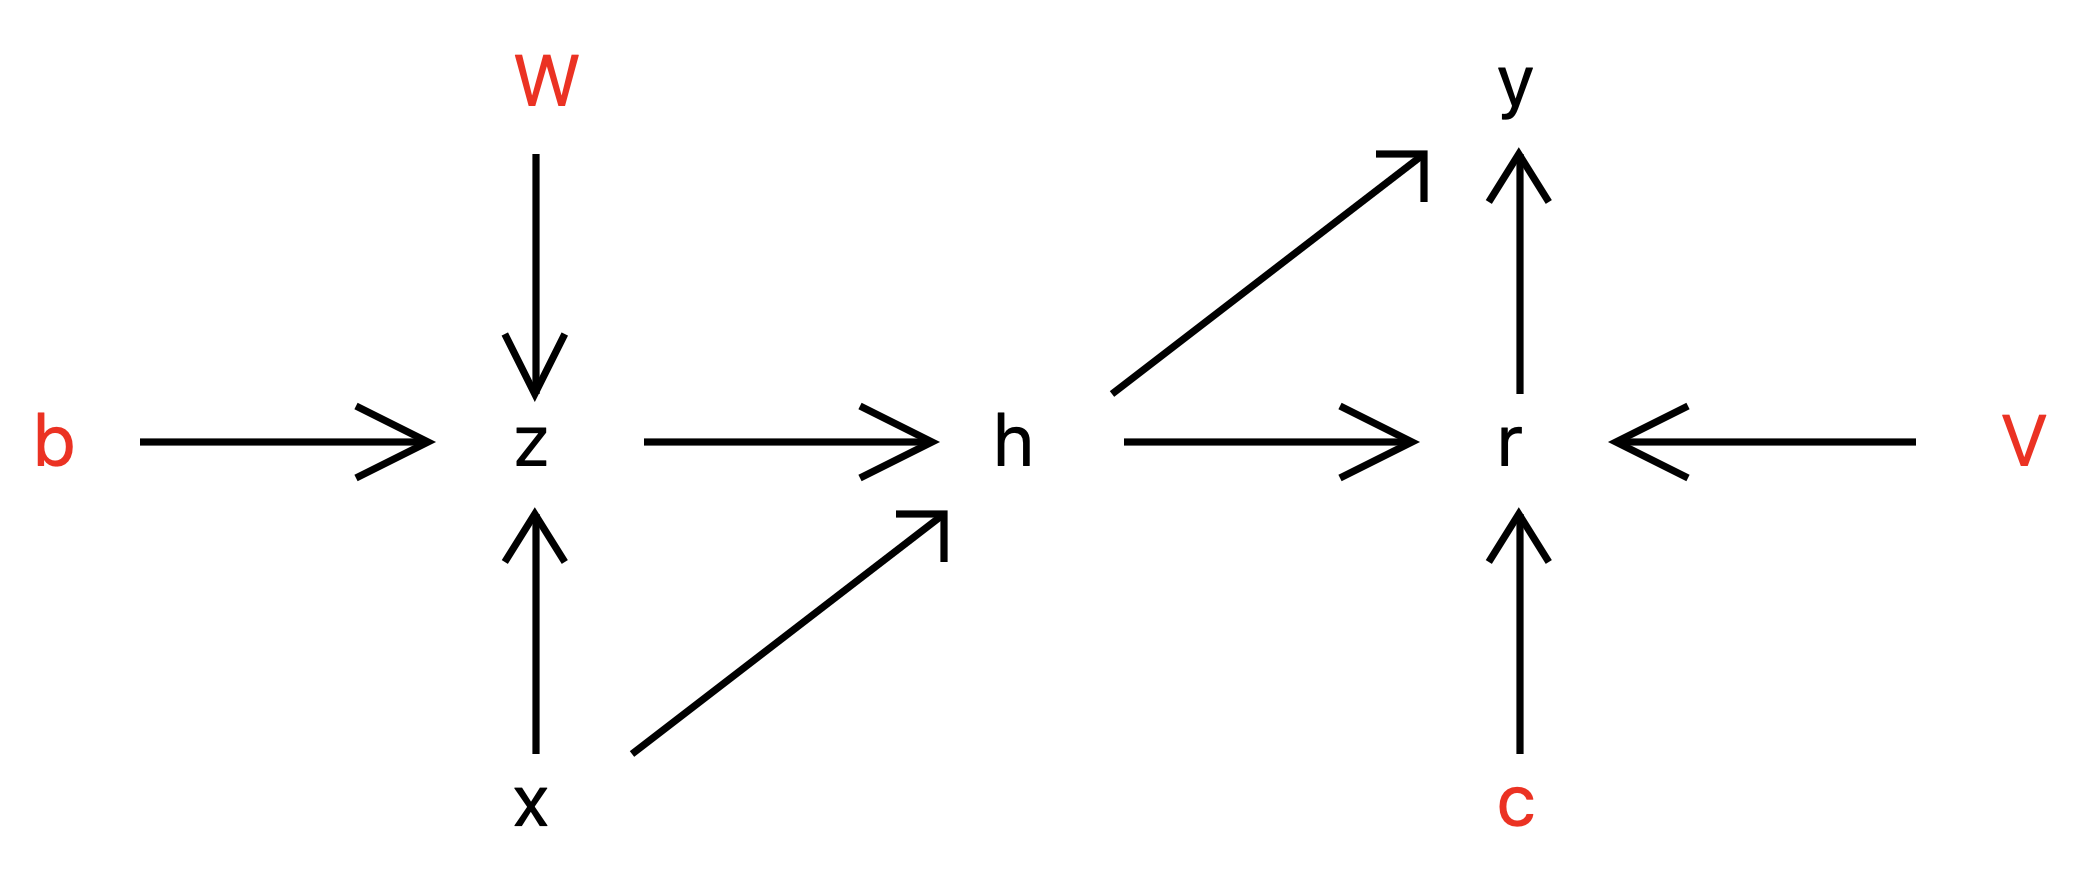
\includegraphics[width=.5\textwidth]{q2.1.png} 
  \caption{The computation graph for all the variables. }
  \label{fig:q2.1}
\end{figure}
\end{homeworkSection}
%%% Subquestion 2
\begin{homeworkSection}
Determine the backprop rules (in vector form) for computing the gradients with respect to all the parameters. 
\\
\begin{gather*}
\begin{aligned}
\textbf{Forward pass: \ \ \ \ } \\
\textbf{z} &= \textbf{Wx} + \textbf{b} \\
\textbf{h} &= \phi(\textbf{z}) + \textbf{x} \\
\textbf{r} &= \textbf{Vh} + \textbf{c} \\
\textbf{y} &= \phi(\textbf{r}) + \textbf{h} \\
%\end{aligned}
%\end{gather*}
\textbf{Backward pass: \ \ \ \ } \\
%\begin{gather*}
%\begin{aligned}
\overline{\textbf{y}} &= \textbf{1} \\
\overline{\textbf{r}} &= \overline{\textbf{y}} \cdot \frac{\partial\textbf{y}}{\partial\textbf{r}} = \phi'(\textbf{r}) \\
\frac{\partial{\textbf{r}}}{\partial{\textbf{V}}} &= \textbf{1}\textbf{h}^T \\
\frac{\partial{\textbf{r}}}{\partial{\textbf{c}}} &= \textbf{1} \\
\overline{\textbf{V}} &= \textbf{1} \overline{\textbf{r}}^T \cdot \frac{\partial{\textbf{r}}}{\partial{\textbf{V}}} = \textbf{1} \phi'(\textbf{r})^T \cdot \textbf{1}\textbf{h}^T = \textbf{1} [\phi'(\textbf{r}) \cdot \textbf{h}]^T\\
\overline{\textbf{c}} &= \overline{\textbf{r}} \cdot \frac{\partial{\textbf{r}}}{\partial{\textbf{c}}} = \phi'(\textbf{r}) \\
\overline{\textbf{h}} &= \overline{\textbf{y}} \cdot \frac{\partial\textbf{y}}{\partial\textbf{h}} + \overline{\textbf{r}} \cdot \frac{\partial\textbf{r}}{\partial\textbf{h}} = \textbf{1} + \textbf{V} \phi'(\textbf{r}) \\
\overline{\textbf{z}} &= \overline{\textbf{h}} \cdot \frac{\partial\textbf{h}}{\partial\textbf{z}} = \overline{\textbf{h}} \cdot \phi'(\textbf{z}) = \phi'(\textbf{z}) + \textbf{V} \phi'(\textbf{r}) \cdot \phi'(\textbf{z}) \\
\overline{\textbf{W}} &= \textbf{1} \overline{\textbf{z}}^T \cdot \frac{\partial\textbf{z}}{\partial\textbf{W}} = [\textbf{1} \phi'(\textbf{z})^T + \textbf{1} (\textbf{V} \phi'(\textbf{r}) \cdot \phi'(\textbf{z}))^T] \cdot \textbf{1} \textbf{x}^T \\
& = \textbf{1} [\phi'(\textbf{z})^T \cdot \textbf{x}^T + \phi'(\textbf{r})^T \textbf{V}^T \cdot \phi'(\textbf{z})^T \cdot \textbf{x}^T]\\
\overline{\textbf{b}} &= \overline{\textbf{z}} \cdot \frac{\partial\textbf{z}}{\partial\textbf{b}} = [\phi'(\textbf{z}) + \textbf{V} \phi'(\textbf{r}) \cdot \phi'(\textbf{z})] \cdot \textbf{1} \\
\end{aligned}
\end{gather*}
$\textbf{x}$, $\textbf{y}$ and $\textbf{h}$ all have the same size. $\textbf{1}$ is a vector with the same size as $\textbf{y}$, whose each unit is 1. 
\end{homeworkSection}
\end{homeworkProblem}


%% Question 3
\begin{homeworkProblem}
\textbf{AlexNet.}
%%% Subquestion 1
\begin{homeworkSection}
\emph{Count the number of units, the number of weights, and the number of connections in each layer.} \\
\\
% 150,528-253,440-186,624-64,896-64,896-43,264-4096-4096-1000
\begin{tabular}{|r|r r r|}
  \hline 
  & \# Units & \# Weights (Parameters) & \# Connections\\
  \hline  
  Input & 3*224*224=150,528 &  &  \\
  Convolution Layer 1 & 96*55*55=290,400& 11*11*3*96=34,848  & 11*11*3*96*55*55=105,415,200 \\
  Pooling Layer & 96*27*27=69,984 &  &  \\
  Convolution Layer 2 & 256*27*27=186,624 & 5*5*48*128*2=307,200 & 5*5*48*128*27*27=111,974,400 \\
  Pooling Layer & 256*13*13=43,264 &  &  \\
  Convolution Layer 3 & 384*13*13=64,896 & 3*3*256*384=884,736 & 3*3*256*384*13*13=149,520,384 \\
  Convolution Layer 4 & 384*13*13=64,896 & 3*3*192*192*2=663,552 & 3*3*129*384*13*13=112,140,288 \\
  Convolution Layer 5 & 256*13*13=43,264 & 3*3*192*128*2=442,368 & 3*3*192*256*13*13=74,760,192 \\
  Pooling Layer & 256*6*6=9,216 &  &  \\
  Fully Connected Layer 1 & 4,096 & 9216*4096=37,748,736 & 9216*4096=37,748,736 \\
  Fully Connected Layer 2 & 4,096 & 4096*4096=16,777,216 & 4096*4096=16,777,216 \\
  Output Layer & 1,000 & 4096*1000=4,096,000 & 4096*1000=4,096,000 \\
  \hline  
\end{tabular}
\\
\\
Layers 2, 4 \& 5 are not connected to layers between GPUs; thus, we calculate the parameters and connections of each component and multiplied by 2. 
\end{homeworkSection}
%%% Subquestion 2
\begin{homeworkSection}	
\emph{For each of the following scenarios, based on your answers to Part 1, suggest a change to the architecture which will help achieve the desired objective. I.e., modify the sizes of one or more layers.} \\
\\
\textbf{i.} You want to reduce the memory usage at test time so that the network can be run on a cell phone; this requires reducing the number of parameters for the network.
\\
\\
\textbf{ii.} Your network will need to make very rapid predictions at test time. You want to reduce the number of connections, since there is approximately one add-multiply operation per connection.

\end{homeworkSection}
\end{homeworkProblem}


\end{document}

%\begin{gather*}
%\end{gather*}







